\documentclass[10pt]{standalone}
\usepackage[sc]{mathpazo}
\usepackage{commands}

\begin{document}
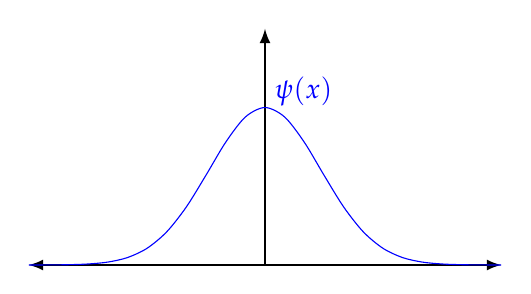
\begin{tikzpicture}
    \draw[thick, latex-latex] (-3, 0) -- (3, 0);
    \draw[thick, -latex] (0, 0) -- (0, 3);
    \draw[scale=1, domain=-3:3, smooth, variable=\x, blue]  plot ({\x}, {2*exp(-(\x)^2)});
    \node[right, blue] at (0, 2.2) {$\psi(x)$};
\end{tikzpicture}
\end{document}